%% ==========================================================================
\section{Background: high-school algebra}
%% ==========================================================================

\begin{frame}
  \frametitle{Vectors in $\Rset^n$}
  \framesubtitle{Definition and Basics}

   A vector $\bx\in\Rset^d$ is defined by a $d$-uplet $(x_1, x_2, \dots, x_d)$, \textit{its coordinates}.

  \begin{block}{Elementary operations}
  \vspace{-.5cm}
  \begin{multicols}{2}
   \begin{itemize}
    \item Addition of two vectors (define a parallelogram)
    \begin{equation*}
    \bx + \by = \begin{pmatrix}
    x_1 + y_1 \\ x_2 + y_2 \\ \vdots \\ x_d + y_d
    \end{pmatrix}
  \end{equation*}
    \item Multiplication by a scalar (streching)
   \end{itemize}
  \begin{equation*}
    \lambda \bx = \begin{pmatrix}
    \lambda x_1 \\ \lambda x_2 + c \\ \vdots \\ \lambda x_d
    \end{pmatrix}, \quad \lambda, c \in \Rset.
  \end{equation*}
  \end{multicols}
  \end{block}

  \begin{block}{Properties}
  \vspace{-.5cm}
  \begin{multicols}{2}
    \begin{itemize}
      \item associativity: $(\bx + \by) + \bz = \bx + (\by + \bz)$
      \item commutativity: $\bx + \by = \by + \bx$
      \item linearity: $\lambda (\bx + \by) = \lambda \bx + \lambda \by$
      \item $(\lambda_1 + \lambda_2) \bx = \lambda_1\bx + \lambda_2 \bx$
    \end{itemize}  
  \end{multicols}
  \end{block}
  
\end{frame}

\begin{frame}
  \frametitle{Vectors in $\Rset^n$}
  \framesubtitle{Dot/Inner product and norm}

  \begin{block}{Dot product of 2 vectors: \textcolor{black}{sum of the products between each coordinate:}}
  \vspace{-.25cm}
  \begin{equation*}
    \langle \bx, \by \rangle \equiv \bx \cdot \by \equiv \bx^\top \by \triangleq \sum_{i=1}^d x_i \, y_j.
  \end{equation*}
  \begin{multicols}{2}
  \begin{itemize}
    \item $\bx^\top \by = \by^\top \bx$
    \item $\bx^\top (\by + \bz) = \bx^\top \by + \bx^\top \bz$
    \item $\lambda (\bx^\top \by) = (\lambda (\bx)^\top \by = \bx^\top (\lambda \by) $
    \item if $\bx = \bzero$, then $\bx^\top \bx = 0$.
  \end{itemize}
  \end{multicols}
  \end{block}

  \begin{block}{(Euclidean) norm (a.k.a length, magnitude) } 
  \vspace{-.35cm}
    \begin{equation*}
      \| \bx \| = \sqrt{\bx^\top \bx}. \quad \textrm{we have }   \| \lambda \bx \| = |\lambda| \| \bx \|.
    \end{equation*}
  \end{block}

\end{frame}

\begin{frame}
  \frametitle{Vectors in $\Rset^n$}
  \framesubtitle{Distances and orthogonality}

  \begin{block}{(Euclidean) distance between 2 vectors} 
    \begin{equation*}
      \distance(\bx, \by) = \| \bx - \by \|.
    \end{equation*}
  \end{block}

  \pause
  
  Remark that when $\bx$ and $\by$ are orthogonal and non zero, distances between $\bx$ and $\by$ and $\bx$ and $(-\by)$ are the same. Then, 
  \begin{equation*}
    (\bx - \by)^\top(\bx - \by) = (\bx + \by)^\top(\bx + \by) \Leftrightarrow \bx^\top\by  = 0,
  \end{equation*}
  
  which motivates the following definition of orthornality:
  \begin{block}{Orthogonality}
  Two vectors $\bx, \by \neq \bzero$ are orthogonal iff $\bx^\top \by = 0$.
  \end{block}

\end{frame}


\begin{frame}
  \frametitle{Vectors in $\Rset^n$}
  \framesubtitle{Orthogonal Projection and geometric definition of the dot product}

  \begin{columns}
  \begin{column}{.5\textwidth}
  \begin{block}{Orthogonal projection of $\bx$ onto $\by$}
    It is the vector $\bz$ such that
  \begin{enumerate}
    \item $\bz = \lambda \by$
    \item $\by$  is orthogonal to $\bx - \bz$
  \end{enumerate}
    We find $\lambda =\bx^\top \by / \|\by \|^2 $ 
  \end{block}
  \end{column}
  \begin{column}{.5\textwidth}
    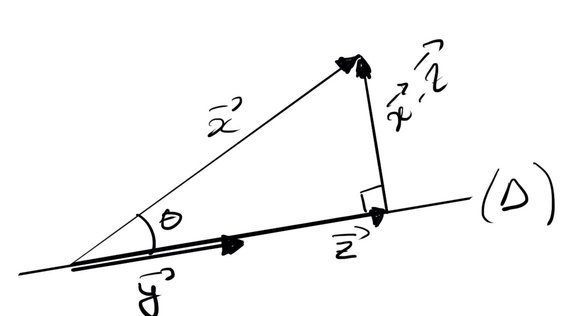
\includegraphics[width=\textwidth]{scalar_projection}
  \end{column}
  \end{columns}

  \pause
  Thanks to Pythagoras theorem, 
  \begin{equation*}
    \cos(\theta) = \frac{\|\bz\|}{\|\bx\|} = \lambda \frac{\|\by\|}{\|\bx\|}
  \end{equation*}
  and then we end with the following geometric definition of the dot product
  
  \begin{block}{Dot product: geometric definition} 
  \vspace{-.35cm}
    \begin{equation*}
      \bx^\top \by = \cos (\theta) \| \bx \| \,  \| \by \| 
    \end{equation*}
  \end{block}


\end{frame}
